
\documentclass{standalone}

\usepackage{pgf}
\usepackage{tikz}
\usetikzlibrary{arrows,automata,matrix}
\usepackage[latin1]{inputenc}
\begin{document}
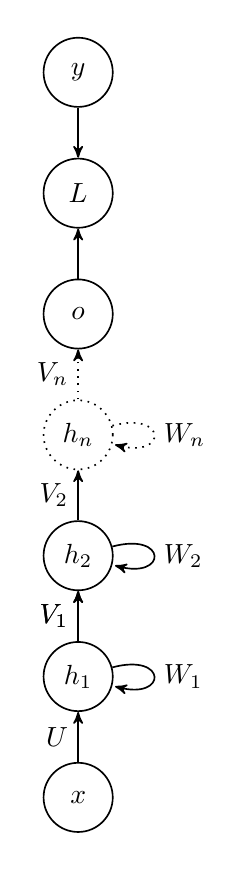
\begin{tikzpicture}[->,>=stealth',shorten >=0pt,auto,node distance=2.8cm,
  semithick]
  \tikzstyle{every state}=[]

  \matrix (m) [matrix of nodes
  ,row sep=.25in,column sep=.25in] {
    \node[state](y) {$y$}; \\
    \node[state](L) {$L$}; \\
    \node[state](o) {$o$}; \\
    \node[state,dotted](hn) {$h_n$}; \\
    \node[state](h2) {$h_2$}; \\
    \node[state](h1) {$h_1$}; \\
    \node[state](x) {$x$}; \\
  };

  \path
  (x) edge    node {$U$} (h1)
  (h1) edge [loop right] node {$W_1$} (h1)
  (h2) edge [loop right] node {$W_2$} (h2)
  (h1) edge  node {$V_1$} (h2)
  (h1) edge  node {$V_1$} (h2)
  (h2) edge  node {$V_2$} (hn)
  (o) edge  node {} (L)
  (y) edge  node {} (L)
  ;
  \path [dotted] 
  (hn) edge  node {$V_n$} (o)
  (hn) edge [loop right] node {$W_n$} (hn)
  ;
  
\end{tikzpicture}

\end{document}